\documentclass[12pt]{article}
\usepackage[utf8]{inputenc}	% Para caracteres en español
\usepackage{amsmath,amsthm,amsfonts,amssymb,amscd}
\usepackage{multirow,booktabs}
\usepackage[table]{xcolor}
\usepackage{fullpage}
\usepackage{lastpage}
\usepackage{enumitem}
\usepackage{fancyhdr}
\usepackage{hyperref}
\usepackage{mathrsfs}
\usepackage{wrapfig}
\usepackage{setspace}
\usepackage{calc}
\usepackage{natbib}
\usepackage{multicol}
\usepackage{cancel}
\usepackage[retainorgcmds]{IEEEtrantools}
\usepackage[margin=3cm]{geometry}
\usepackage{amsmath}
\newlength{\tabcont}
\setlength{\parindent}{0.0in}
\setlength{\parskip}{0.05in}
\usepackage{empheq}
\usepackage{framed}
\usepackage[most]{tcolorbox}
\usepackage{xcolor}
\usepackage{wrapfig,graphicx}
\colorlet{shadecolor}{orange!15}
\parindent 0in
\parskip 12pt
\geometry{margin=1in, headsep=0.25in}
\theoremstyle{definition}
\newcommand{\pd}[2]{\frac{\partial {#1}}{\partial {#2}}}
\newcommand{\mytilde}{\raise.17ex\hbox{$\scriptstyle\mathtt{\sim}$}}
\newtheorem{defn}{Definition}
\newtheorem{reg}{Rule}
\newtheorem{exer}{Exercise}
\newtheorem{note}{Note}
\begin{document}

\thispagestyle{empty}

\begin{center}
{\LARGE \bf Stability and Bifurcations}\\
{\large Prof. Alex Robel}\\
\end{center}

\begin{center}
\color{red}{For an accessible and supremely useful review of linear stability analysis, bifurcations and dynamical systems theory broadly, see ``Nonlinear Dynamics and Chaos'' by Strogatz. These ideas are not just useful in this class, but will help you see a range of scientific problems from a new perspective.}
\end{center}

Some definitions: \\
\begin{itemize}
\item \textbf{Dynamical system (or just ``system''):} One or more differential equations which describe changes in variables over time (and potentially space).
\item \textbf{System state:} A particular set of values of system variables at a particular point in time.
\item \textbf{Fixed point:} A system state for which the rate of change (absent a change in parameters) is zero.
\item \textbf{Limit cycle:} A system state with an oscillatory mode.
\item \textbf{Stability:} A property of a system state which quantifies whether perturbations to the system state cause the system to evolve back to it's original state (stable), or evolve away from the original state (unstable), or not evolve at all following the perturbation (neutral).
\end{itemize}

\section{Linear stability analysis}
Linear stability analysis is a mathematical tool for determining whether a particular system state is stable (will return to a nearby state upon being perturbed) or unstable (will move away to a distance distance system state upon being perturbed).

This tool is ``linear'' in that we take the system equations (which may be very nonlinear) and linearize them to determine the rate of change for small perturbations to the system state. So, consider a generic system in terms of a single variable, $x$
\begin{equation}
\frac{dx}{dt} = f(x)
\end{equation}
where $f(x)$ is some function which may be complicated. A linear stability analysis for this system has three steps:
\begin{enumerate}
\item Determine the fixed points of this system which we call $x_*$. The fixed points are the solution to the equation $f(x_*)=0$.
\item Linearize the system by calculating the derivative of $f(x)$ in terms of the system variable (we will briefly consider how this works for a system with many variables below): $\pd{f}{x}$.
\item Evaluate the derivative $\pd{f}{x}$ at the fixed points: $\pd{f}{x}|_{x=x_*}$. 
\begin{itemize}
\item Where $\pd{f}{x}|_{x=x_*}<0$, the system is stable (i.e. perturbations to the fixed point return to the fixed point)
\item Where $\pd{f}{x}|_{x=x_*}>0$, the system is unstable (i.e. perturbations to the fixed point evolve away from the fixed point)
\item Where $\pd{f}{x}|_{x=x_*}=0$, the system is neutral (i.e. perturbations to the fixed point don't evolve further)
\end{itemize}
\end{enumerate}

The reason why linear stability analysis works, is because the linearization (step 2 in the above list) allows us to write any system (e.g. the example above) as the following linear system
\begin{equation}
\frac{dx'}{dt} = \lambda x'
\end{equation}
where $x' = x-x_*$ and $\lambda = \pd{f}{x}|_{x=x_*}$ from step 2 of the stability analysis. This linear system has a known exponential solution:
\begin{equation}
x'(t) = x'_0 e^{\lambda t}
\end{equation}
where $x'_0 = x'(t=0)$. We can see that when $\lambda<0$, it decays towards the fixed point, and when $\lambda>0$, it exponentially moves away from the fixed point.

We will consider some canonical examples of linear stability analysis in the next section.

\section{Bifurcations}
\textbf{A bifurcation occurs when a change in a parameter causes a change in the stability of a system.} Put in more general terms, a bifurcation is when some prescribed change in the system environment causes a change in the qualitative behavior of the system. Typically, the location of a bifurcation in parameter and system state space is determined by examining where the linear stability of the system crosses through zero, as a function of change in some system parameter. 

In popular parlance, bifurcations are sometimes referred to as ``tipping points''. This term can often be misused, and sometimes is also used to refer to things which aren't bifurcations (i.e. potentially just places where the system state changes rapidly, but doesn't necessarily change stability), so we won't used it here.

In the remainder of this section, we will consider the three most common types of bifurcation that are encountered in simple dynamical systems.

\subsection{Saddle-node (or fold) bifurcation}
In a saddle-node bifurcation, there is originally one stable and one unstable fixed point (and potentially other fixed points), which both meet at the parameter value associated with the bifurcation and then no longer exist beyond that bifurcation point (i.e. they ``annihilate'' each other or are created from seemingly nowhere, which is why this bifurcation is also sometimes called a ``blue sky catastrophe'').

\begin{figure}[h]
  \begin{center}
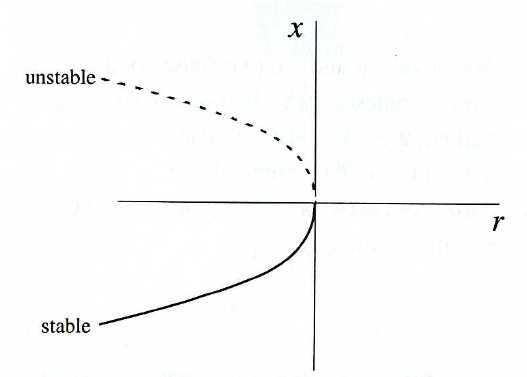
\includegraphics[width=0.5\textwidth]{Saddle_node_bifurcation_diagram.png}
  \end{center}
\end{figure}

\begin{shaded}
\textbf{Example:} Consider the dynamical system (see figure above)
\begin{equation}
\frac{dx}{dt} = r + x^2
\end{equation}
\begin{enumerate}
\item The fixed points are: $x_* = \pm \sqrt{-r}$
\item The linearization is: $\pd{f}{x} = 2x_*$
\item The linear stability at the two fixed points are: $\pd{f}{x} = \pm 2 \sqrt{-r}$. Thus, the positive fixed point ($x_* = \sqrt{-r}$) is unstable and the negative fixed point ($x_* = -\sqrt{-r}$) is stable. The bifurcation where $\pd{f}{x}=0$, and beyond that ($r>0$), there are no fixed point.
\end{enumerate}
\end{shaded}

\subsection{Pitchfork bifurcation}
In a pitchfork bifurcation, there is originally one stable fixed point (and potentially other fixed points), which turns into an unstable fixed point, and two new stable fixed points at the bifurcation point. Another version of the pitchfork bifurcation starts with one unstable fixed point, which then turns into a stable fixed point, and two new unstable fixed points at the bifurcation point.

\begin{figure}[h]
  \begin{center}
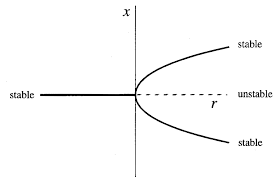
\includegraphics[width=0.5\textwidth]{Pitchfork_bifurcation_diagram.png}
  \end{center}
\end{figure}

\begin{shaded}
\textbf{Example:} Consider the dynamical system (see figure above)
\begin{equation}
\frac{dx}{dt} = rx - x^3
\end{equation}
\begin{enumerate}
\item The fixed points are: $x_* = 0$ and $x_* = \pm \sqrt{r}$
\item The linearization is: $\pd{f}{x} = r - 3x_*^2$
\item The linear stability at the three fixed points are: $\pd{f}{x}|_{x_* = 0} = r$ and $\pd{f}{x}|_{x_* = \pm \sqrt{r}} = -2r$. Thus, the zero fixed point ($x_* = 0$) goes from stable to unstable at the bifurcation ($r=0$) and the other two stable fixed points only exist beyond the bifurcation.
\end{enumerate}
\end{shaded}

\subsection{Hopf bifurcation}
In a Hopf bifurcation, there is originally one stable fixed point (and potentially other fixed points), which turns into an unstable fixed point, and a stable limit cycle. There are two versions of the Hopf bifurcation, which have the difference of whether the stable limit cycle first appears at the bifurcation point (a supercritical Hopf bifurcation) or before the bifurcation point (a subcritical Hopf bifurcation). We will only consider a supercritical Hopf bifurcation here, because it is more common in practice, though there are some interesting glaciological examples of subcritical Hopf bifurcations \cite[i.e.][]{robel-2013:ISvariability}.

\begin{figure}[h]
  \begin{center}
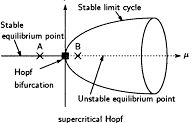
\includegraphics[width=0.5\textwidth]{Hopf_bifurcation_diagram.png}
  \end{center}
\end{figure}

Limit cycles can only occur in system with two or more degrees of freedom (i.e. 2+ variables and 2+ system equations).  To do a linear stability in such a system requires calculating the Jacobian, which is a matrix including all the relevant derivatives for the system of equations. For example, the Jacobian of a two-equation dynamical system: $dx/dt = f_1(x,y), dy/dt = f_2(x,y)$ is 
\begin{equation}
J =
\begin{bmatrix}
  \frac{\partial f_1}{\partial x} & 
    \frac{\partial f_1}{\partial y} \\[1ex] % <-- 1ex more space between rows of matrix
  \frac{\partial f_2}{\partial x} & 
    \frac{\partial f_2}{\partial y} \\[1ex]
\end{bmatrix}
\end{equation}
The exact definition of the linear stability for such a system with more than one degree of freedom is the determinant of the Jacobian. However, if the only thing you want to know if the sign of the linear stability (i.e. if it is stable or unstable), then you can simply calculate the Trace of the Jacobian, which in the above case is simply $\frac{\partial f_1}{\partial x} +  \frac{\partial f_2}{\partial y}$. Examples for such cases can be a bit more algebra, but in practice are not much more difficult than the one-degree-of-freedom case. For the most classical example of a Hopf bifurcation, see \href{https://en.wikipedia.org/wiki/Hopf_bifurcation#Propositions}{this linear stability analysis of the van der Pol oscillator}.

%\bibliography{/Users/arobel3/Dropbox (GaTech)/Docs/refs.bib}
%\bibliographystyle{apalike}

\end{document}